\section{Intermediate Runs}
The following solutions represent example runs of the solvers when given parameters that result in longer run times. These solutions were run with an expected solution time of approximately 1.5 hours. 

\subsection{Stochastic Loads Method}
The Stochastic Loads solver was run with the following argument list: 

\begin{verbatim}
python -m pystruct <<data_file>>  -S3 -i80 -g118 --csv
\end{verbatim}

\noindent Where: 

\begin{itemize}
  \item \codeword{-S3}: Select solution 3: Stochastic Loads Method
  \item \codeword{-i80}: Use a population size of 80. 
  \item \codeword{-g118}: Use a generation count of 118. 
  \item \codeword{--csv}: Generate CSV output for final Pareto Front
\end{itemize}


\subsubsection{Resultant Pareto Front}
Table \ref{tab:pfront_sto_int} shows the design parameters of the members of the Pareto Front generated by this solution run. The Pareto Front is also given graphically in Figure \ref{fig:pfront_sto_int}. 
\begin{table}[!htbp]
	\caption{Members of the Pareto Front generated through Stochastic Loads (Long Run)}
\label{tab:pfront_sto_int}
\centering
\small
\begin{tabular}{|p{1.5cm}p{1.5cm}p{1.4cm}p{2cm}p{2cm}||p{1.5cm}p{1.5cm}|}
\hline
\multicolumn{5}{|c||}{Design Parameters}&\multicolumn{2}{|c|}{Fitness Properties}\\
\hline
Top Flange Width&Bottom Flange Width&Web Thickness&Doubler Thickness at Hoist Pin&Doubler Thickness at Load Pin&Fitness 1& Fitness 2\\
\hline
mm&mm&mm&mm&mm&ul&kg\\
\hline
91.554&162.123&96.774&33.461&85.072&6.476&883.916\\
136.451&174.904&5.769&9.201&82.508&4.048&210.288\\
145.704&60.423&3.758&4.187&141.234&1.147&173.851\\
173.109&82.136&89.105&30.424&192.874&6.440&870.671\\
108.471&224.84&20.092&18.651&126.978&5.613&351.830\\
51.004&196.645&72.695&35.218&157.498&6.401&734.404\\
42.434&142.466&92.231&39.827&255.918&6.553&899.608\\
58.538&239.768&14.161&130.261&20.683&5.060&336.291\\
83.903&245.174&90.334&39.019&155.065&6.644&900.300\\
92.43&264.003&84.446&107.606&213.235&6.678&945.900\\
188.818&243.694&86.99&43.612&216.242&6.707&946.510\\
84.477&163.361&69.605&37.477&197.817&6.358&730.305\\
38.11&211.227&39.013&32.279&117.635&5.897&465.475\\
176.577&242.853&45.056&84.272&162.865&6.289&638.765\\
\hline
\end{tabular}
\end{table}

\begin{figure}
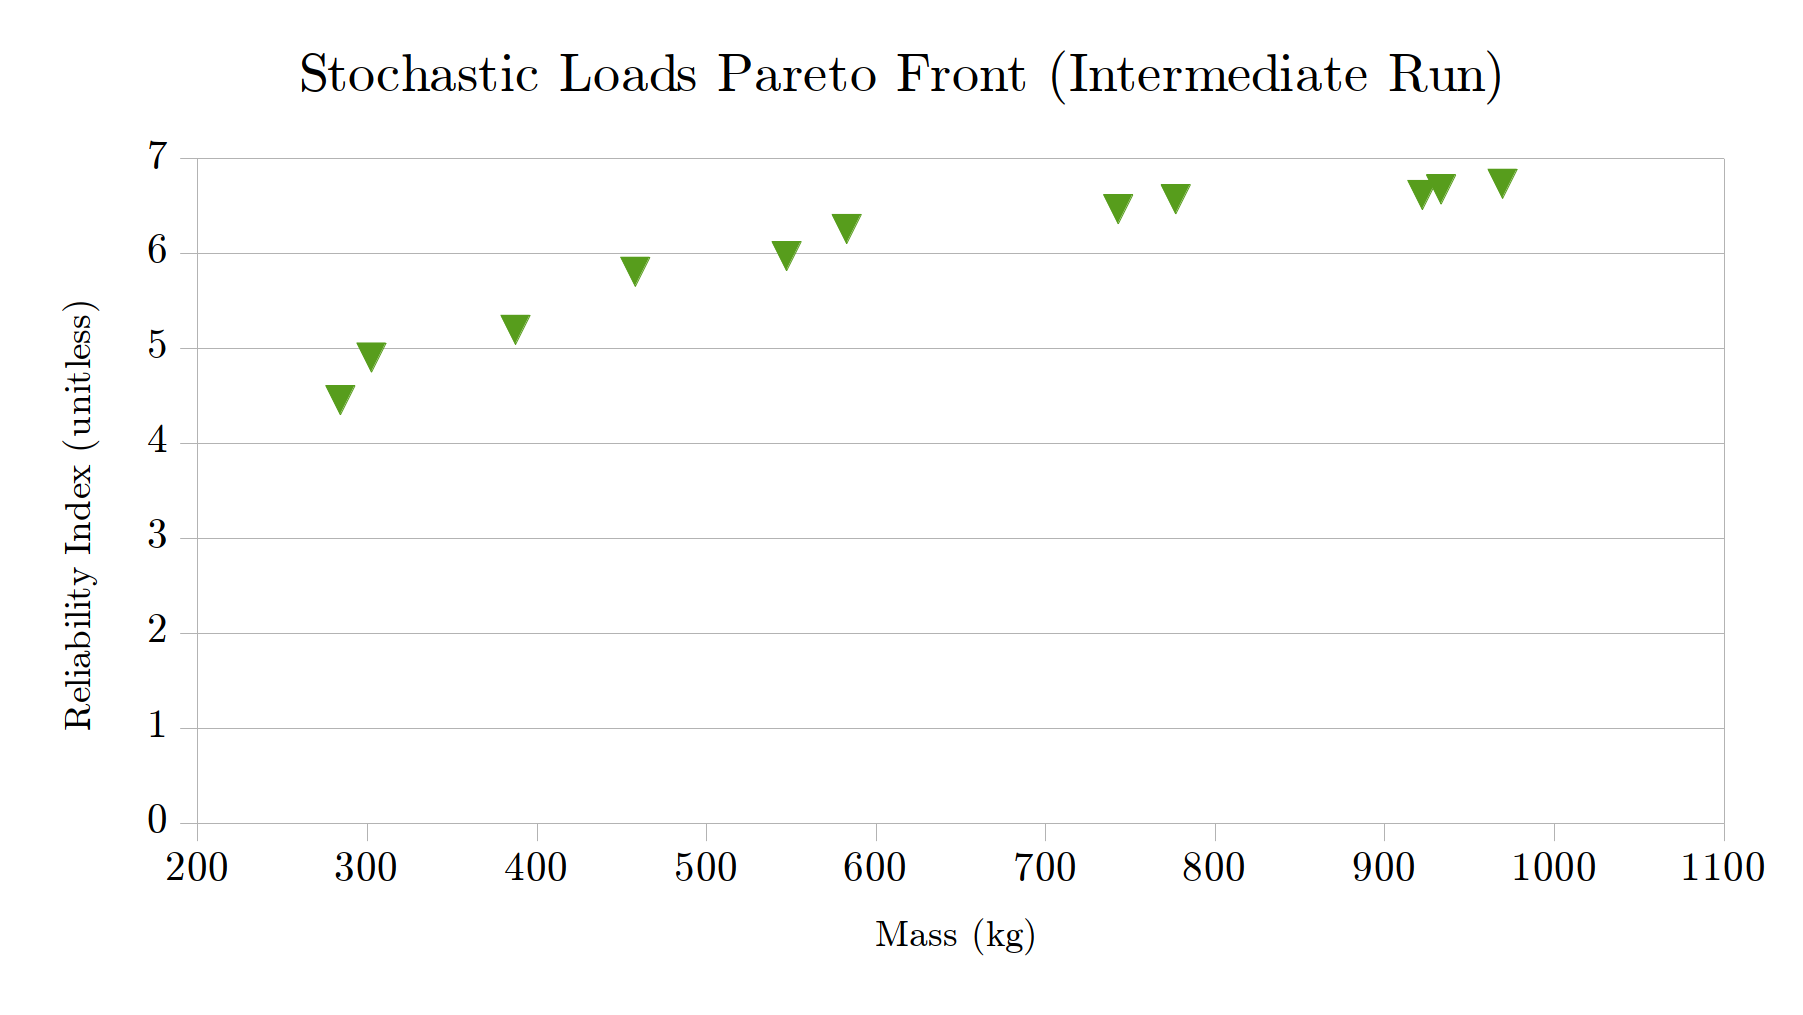
\includegraphics[width=\textwidth]{img/pf_sto_int.png}
	\caption{Graph of the Pareto Front generated through Stochastic Loads (Intermediate Run)}
\label{fig:pfront_sto_int}
\end{figure}

\subsubsection{Solution Statistics}
This solution also was tracked for several computing performance indicators to compare the performance of the algorithm with the other solutions. These statistics are listed in Table \ref{tab:stat_sto_int}. 

\begin{table}[!htbp]
  \caption{Solution Statistics for Stochastic Loads (Intermediate Run)}
  \label{tab:stat_sto_int}
  \centering
  \begin{tabular}{|l|l|}
    \hline
	  Total Generations Computed & 118\\
    Average Time Per Generation (sec) & 44.6\\
    Total Calls to Nastran & 18.9E+03\\
    Total Wall Clock Time (sec)	 & 5.26E+03\\
    \hline
  \end{tabular}
\end{table}




\subsection{Aggregate LHS Method}
This solution was calculated using parameters designed to produce approximately the same wall clock solution time as the Stochastic Loads Long Run. The command line that was used was:

\begin{verbatim}
python -m pystruct <<data_file>>  -S2 -i80 -g10 --csv
\end{verbatim}

\noindent Where: 

\begin{itemize}
  \item \codeword{-S2}: Select solution 2: Aggregate LHS method
  \item \codeword{-i80}: Use a population size of 80. 
  \item \codeword{-g10}: Use a generation count of 10. 
  \item \codeword{--csv}: Generate CSV output for final Pareto Front
\end{itemize}

\subsubsection{Resultant Pareto Front}
Table \ref{tab:pfront_agg_int} shows the design parameters of the members of the Pareto Front generated by this solution run. The Pareto Front is also given graphically in Figure \ref{fig:pfront_agg_int}. 
\begin{table}[!htbp]
\small
\caption{Members of the Pareto Front generated through Aggregated LHS (Intermediate Run)}
\label{tab:pfront_agg_int}
\begin{tabular}{|p{1.5cm}p{1.5cm}p{1.5cm}p{1.4cm}p{2cm}p{2cm}||p{1.5cm}p{1.5cm}|}
\hline
\multicolumn{6}{|c||}{Design Parameters}&\multicolumn{2}{|c|}{Fitness Properties}\\
\hline
Parent Load Case&Top Flange Width&Bottom Flange Width&Web Thickness&Doubler Thickness at Hoist Pin&Doubler Thickness at Load Pin&Fitness 1& Fitness 2\\
\hline
&mm&mm&mm&mm&mm&MPa&kg\\
\hline
0&33.419&225.434&73.378&98.902&168.627&47.853&798.650\\
1&143.545&236.63&28.941&51.856&235.41&64.905&508.344\\
2&19.175&188.212&16.86&30.671&37.477&119.453&248.737\\
3&199.109&254.274&16.579&16.375&86.75&82.816&355.258\\
3&33.363&247.127&25.562&69.85&151.036&78.490&421.570\\
5&121.908&223.483&36.019&33.132&137.859&64.943&491.084\\
7&221.559&182.211&66.899&50.441&239.791&47.342&800.844\\
7&128.846&235.091&91.383&56.015&237.029&38.693&970.085\\
8&105.514&234.267&22.39&17.883&88.972&83.876&354.867\\
9&78.813&241.044&64.019&57.815&149.831&49.530&713.439\\
11&196.067&244.277&75.958&52.973&207.994&41.252&871.485\\
12&132.607&201.494&11.377&11.854&55.446&116.316&251.795\\
13&90.794&182.028&10.874&61.727&40.795&112.348&256.324\\
13&203.108&242.266&69.082&54.453&184.526&43.916&813.627\\
13&96.629&220.072&91.25&83.831&231.002&39.842&969.358\\
13&195.498&230.446&10.287&26.793&52.834&88.207&291.272\\
13&13.753&183.011&32.323&19.896&204.089&82.393&421.370\\
15&146.586&223.616&26.394&80.044&124.2&71.861&460.528\\
15&152.869&237.926&47.014&26.381&109.515&56.971&573.852\\
15&34.014&246.74&71.006&33.891&199.994&49.218&752.078\\
18&156.168&256.859&43.914&85.261&213.37&54.567&649.804\\
18&205.308&209.455&68.848&69.806&139.258&49.101&792.489\\
20&167.288&235.526&38.693&51.83&157.507&59.123&557.048\\
23&244.161&222.004&18.401&65.974&117.95&75.055&426.038\\
23&152.862&224.748&15.939&70.565&54.526&84.558&348.899\\
23&197.734&237.684&70.884&46.01&156.049&44.353&804.368\\
\hline
\end{tabular}
\end{table}

\begin{figure}[!htbp]
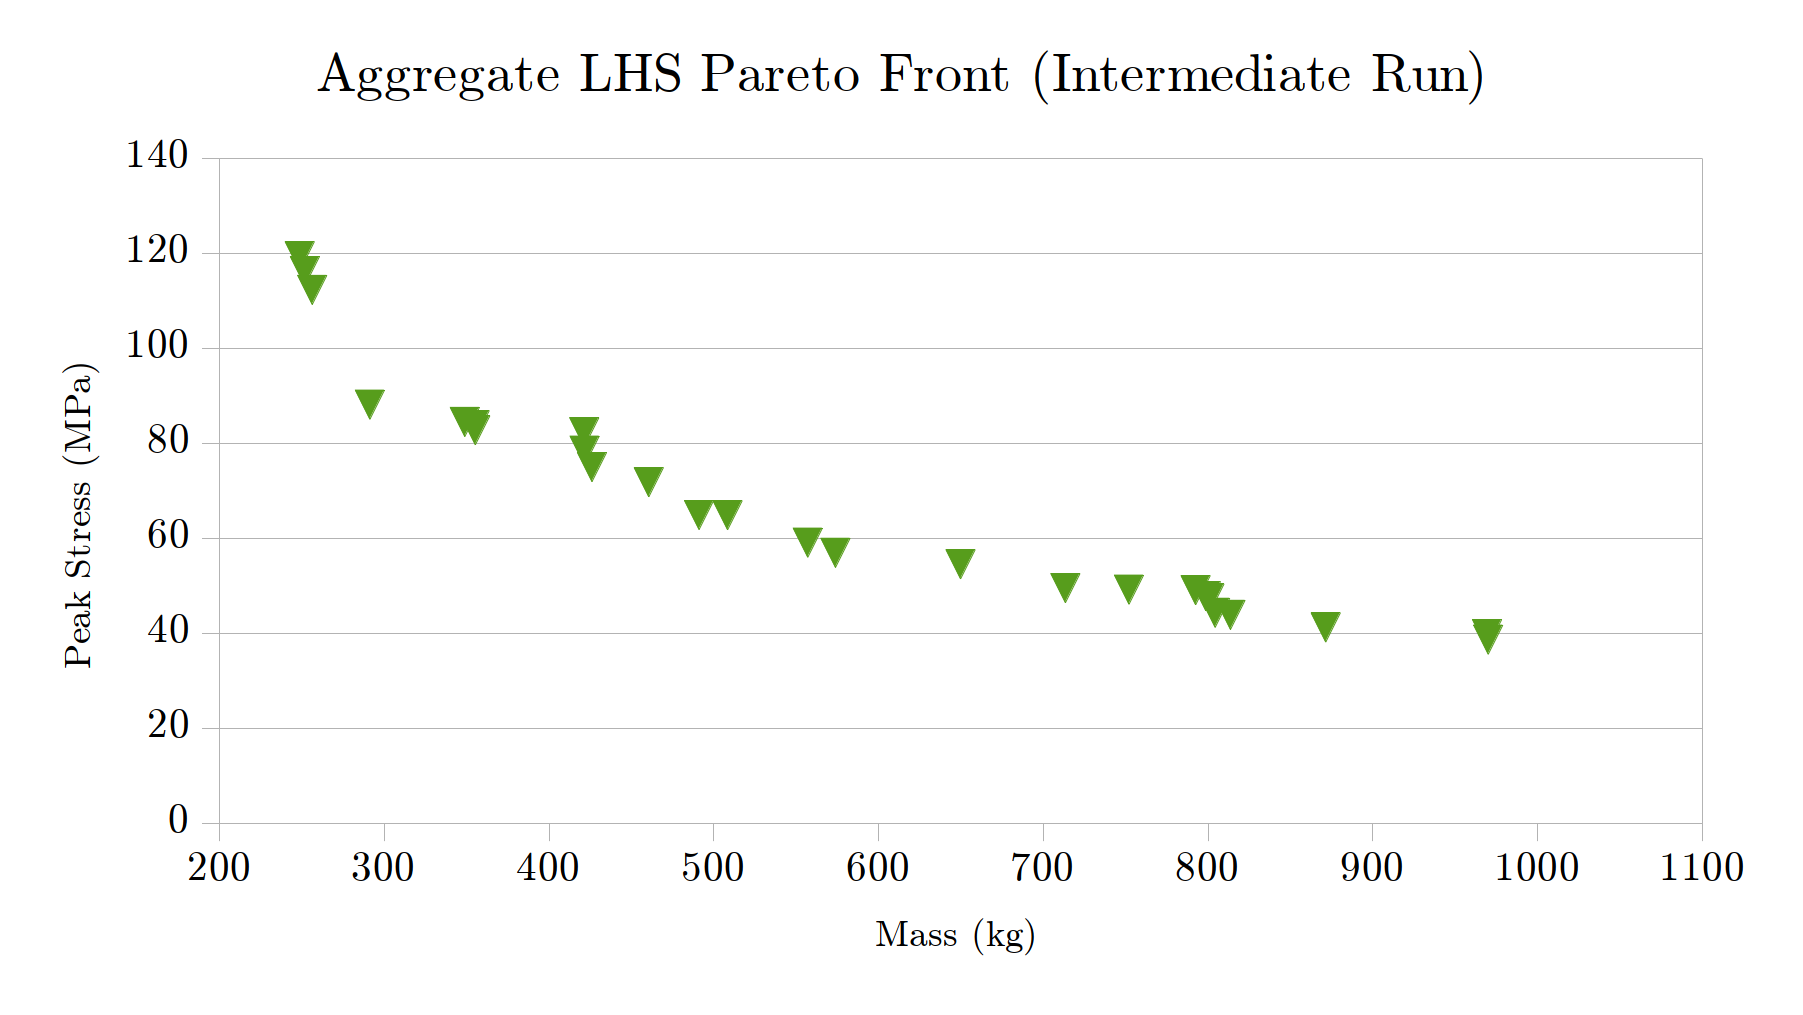
\includegraphics[width=\textwidth]{img/pf_agg_int.png}
\caption{Graph of the Pareto Front generated through Aggregated LHS (Intermediate Run)}
\label{fig:pfront_agg_int}
\end{figure}

\subsubsection{Solution Statistics}
This solution also was tracked for several computing performance indicators to compare the performance of the algorithm with the other solutions. These statistics are listed in Table \ref{tab:stat_agg_int}. 

\begin{table}[!htbp]
  \centering
\caption{Solution Statistics for Aggregated LHS (Intermediate Run)}
  \label{tab:stat_agg_int}
  \begin{tabular}{|l|l|}
    \hline
	  Total Generations Computed & 250\\
    Average Time Per Generation (sec) & 21.2\\
    Total Calls to Nastran & 20E+03\\
    Total Wall Clock Time (sec)	 & 5.30E+03\\
    \hline
  \end{tabular}
\end{table} 

